\documentclass[12pt, ngerman]{scrartcl}   %scrartcl, scrreprt; option parskip für Absatz mit Abstand statt Einzug
\usepackage[utf8]{inputenc}
\usepackage[T1]{fontenc}
\usepackage[ngerman]{babel}
\usepackage{graphicx}
\usepackage[locale = DE,separate-uncertainty = true]{siunitx}
\usepackage{amsmath, mathtools, amssymb, amsthm}
\usepackage{enumitem}
\usepackage[version=4]{mhchem}
\usepackage[left=3cm,right=2cm,top=2cm,bottom=2cm]{geometry} %stehpan
\usepackage{lmodern}    %Schriftart, benötigt für microtype
\usepackage{textcomp}
\usepackage{microtype}  %schöneres Schriftbild
\usepackage{caption}
\usepackage{graphicx}
\usepackage{subcaption}
\usepackage{longtable}  %Tabellen mit Seitenumbruch usw
\usepackage{threeparttable}
\usepackage{dcolumn}    %In Tabelle nach Komma Ausrichten
\usepackage{multirow}   %für Tabellen
\usepackage[hidelinks]{hyperref}
\usepackage[sorting = none, maxbibnames=5]{biblatex}
\usepackage[babel, german=quotes]{csquotes}   %empfohlen für Biblatex
\usepackage{float}      %für Positionierungsoption H
\usepackage[section]{placeins}
\usepackage[onehalfspacing]{setspace}
\usepackage{smartdiagram}   %flowcharts ect.
\usepackage{wrapfig}
\usepackage{listings}
\usepackage{booktabs}
\usepackage{mhchem}
\usepackage[headsepline]{scrlayer-scrpage}
\usepackage{pgfplots}
\usepackage{physics}
\usepackage[export]{adjustbox}
\numberwithin{equation}{section}
\usepackage[acronym,toc]{glossaries} %stehpan
\usepackage{cite} % Verbessertes Zitieren
\usepackage{fancyhdr}

\bibliography{literatur}
\setcounter{biburllcpenalty}{9000}  %verhindert, dass urls über den Rand gehen
\setlength{\parindent}{0pt}
\sisetup{separate-uncertainty}   %Einheiten als Potenz, separate-uncertainty für Fehler mit +/-

\pagestyle{scrheadings}
\clearpairofpagestyles
\automark{section}
\ohead{\pagemark}
\ihead{\scshape \rightmark}

% Keine "Schusterjungen"
\clubpenalty = 10000
% Keine "Weisen"
\widowpenalty = 10000 \displaywidowpenalty = 10000

\definecolor{mygreen}{rgb}{0,0.6,0}
\lstset{
    language = python,
    tabsize = 4,
    frame = single,
    rulecolor = \color{black},
    breaklines = true,
    showstringspaces = false,
    basicstyle = \small\ttfamily\singlespacing,
    commentstyle = \color{mygreen},
}


\tikzset{every label/.style={font=\scriptsize,inner sep=1pt}}
\newcommand{\stencilpt}[4][]{\node[circle,fill,draw,inner sep=2pt,label={above left:#4},#1] at (#2) (#3) {}}
\AtBeginDocument{\RenewCommandCopy\qty\SI} 
\pgfplotsset{compat=1.18,width=0.8\linewidth}
\DeclareSIUnit \parsec {pc}

\begin{document}


\begin{center}

\begin{LARGE}
\textbf{Untersuchung der Abschirmung von kosmischen Myonen und dessen Einfluss auf die Zählrate mit dem MuPix 8 Sensor  } \\ 
\end{LARGE}

\vspace{40mm}

\begin{Large}

Bachelorarbeit

\vspace{\baselineskip}

in dem Fach\\
Physik\\


\vspace{\baselineskip}

an der Fakultät für  Physik und Astronomie\\
an der Ruhr-Universität Bochum
\vspace{2\baselineskip}

von\\
Jonas Goedert\\
\vspace{\baselineskip}

aus\\
Essen
\vspace{2\baselineskip}

Bochum (\the\year{})

\end{Large}

\end{center} 
\thispagestyle{empty}
\clearpage



\input{Abstrakt}
\clearpage

\tableofcontents
\thispagestyle{empty}
\newpage


\section{Motivation}
Der MuPix8 Sensor wurde ursprünglich für das Mu3e-Experiment entwickelt und wird in Zukunft auch Anwendung in dem $\overline{P}$ANDA-Experiment am Beschleunigunszentrum FAIR haben. 
Jedoch lässt sich der MuPix8 auch als Myonendetektor verwenden, was ihn somit interessant für die Methode der Myonentomografie macht. 
Diese bedient sich kosmischer Myonen welche in der Lage sind mehrere Kilometer an Fels zu durchdringen. 
Es kann sowohl die Absorption, als auch die Coulomb-Streuung der Myonen durch das Absorbermaterial beobachtet werden um selbst von großen Objekten oder Gesteinsschichten ein Bild zu erhalten. 
Diese Art um die Struktur und Zusammensetzung von Objekten zu studieren wird bereits in der Archäologie und der Untersuchung von Vulkanen verwendet und soll bald auch seinen Einsatzt in der Geothermie finden. \\
\newline
Diese Arbeit beschäftigt sich damit, in wie weit der MuPix8 Sensor für diese Aufgabe geeignet ist. 
Es wird die Absorption von Myonen, durch Blei untersucht um festzustellen ob bereits bekannte Phänomene in der  Detektion von Myonen Reproduziert werden können. 


\clearpage


\section{Theoretische Grundlagen} \label{grundlagen}

\subsection{Standartmodell der Teilchenphysik} \label{standartmodell}
Das Standardmodell der Teilchenphysik ist eine theoretische Beschreibung der fundamentalen Bausteine der Materie und ihrer Wechselwirkungen.
Materie und Wechselwirkung kommen von drei Elementarteilchen, die Leptonen, Quarks und Bosonen. 
Leptonen und Quarks werden auch als Fermionen bezeichnet und haben einen Spin von $1/2$. 
Ebenfalls unterscheidet man zwischen drei Generationen von Leptonen und Quarks. 
Die Quarks unterscheiden sich in ihrem \textit{flavour}. 
Somit gibt es das up, down, charm, strange, top und bottom Quark. 
Desweiteren tragen Quarks die so genannte Farbladung.
Hier wird unterschieden zwischen rot, grün und blau, so wie den entsprechenden Antifarben. 
Die Leptonen treten, wie bereits erwähnt auch in drei Generationen auf. 
Jede Generation besteht aus einem Teilchen und dem dementsprechenden Neutrino. 
Die erste Generation umfasst das Elekktron $e^{-}$ und das Elektron-Neutrino $\nu_e$, die zweite Generation das Myon und das Myon-Neutrino $\nu_{\mu}$ und die dritte Generation das Tau $\tau$ so wie das Tau-Neutrino $\nu_{\tau}$.\\
\newline 
Die Bosonen sind die Vermittler der Wechselwirkungen. 
Bosonen haben einen ganzzahligen Spin und beseitzen, bis auf das W Boson $W\pm$, keine Ladung. 
So ist das Photon für die Übertragung der elektromagnetischen Wechselwirkungen,das W und Z Boson für die schwache Wechselwirkung und das Gluon für die starke Wechselwirkungen verantwortlich. 
Bei der starken Wechselwirkung kommen die Farbladungen wieder ins Spiel. 
Die starke Wechselwirkung bindet die Quarks zu Hardonen wie Protonen oder Neutronen, welche wiederum zu den Bayronen zählen zusammen.
Baryonen bestehen aus drei Quarks, Mesonen, welche auch zu den Hadronen zählen, setzten sich aus einem Quark und dem entsprechenden Anti-Quark zusammen. 
Sowohl Baryonen als auch Mesonen müssen immer farbneutral sein, man sagt auch sie sind "weiß". 
Das bedeutet, dass die Quarks welche das jeweilige Teilchen ausmachen, zusammen "weiß" ergeben. 
Dies erhält man wenn, die drei Quarks jeweils die Farbe rot, grün und blau haben, oder wenn wenn ein Quark mit einer Farbe und das Antiquark mit der entsprechenden Anti-Farbe gebunden sind.
Man spricht hier auch vom sogenannten Confinement. \\
Das letzte Boson, das Higgs-Boson, welches nach langer Suche am CERN gefunden wurde, ist jenes Elementarteilchen, was allem seine Masse verleiht. Auch das Higgs-Boson hat keine Ladung aber auch einen Spin von 0.

\begin{figure}[h]
    \centering
    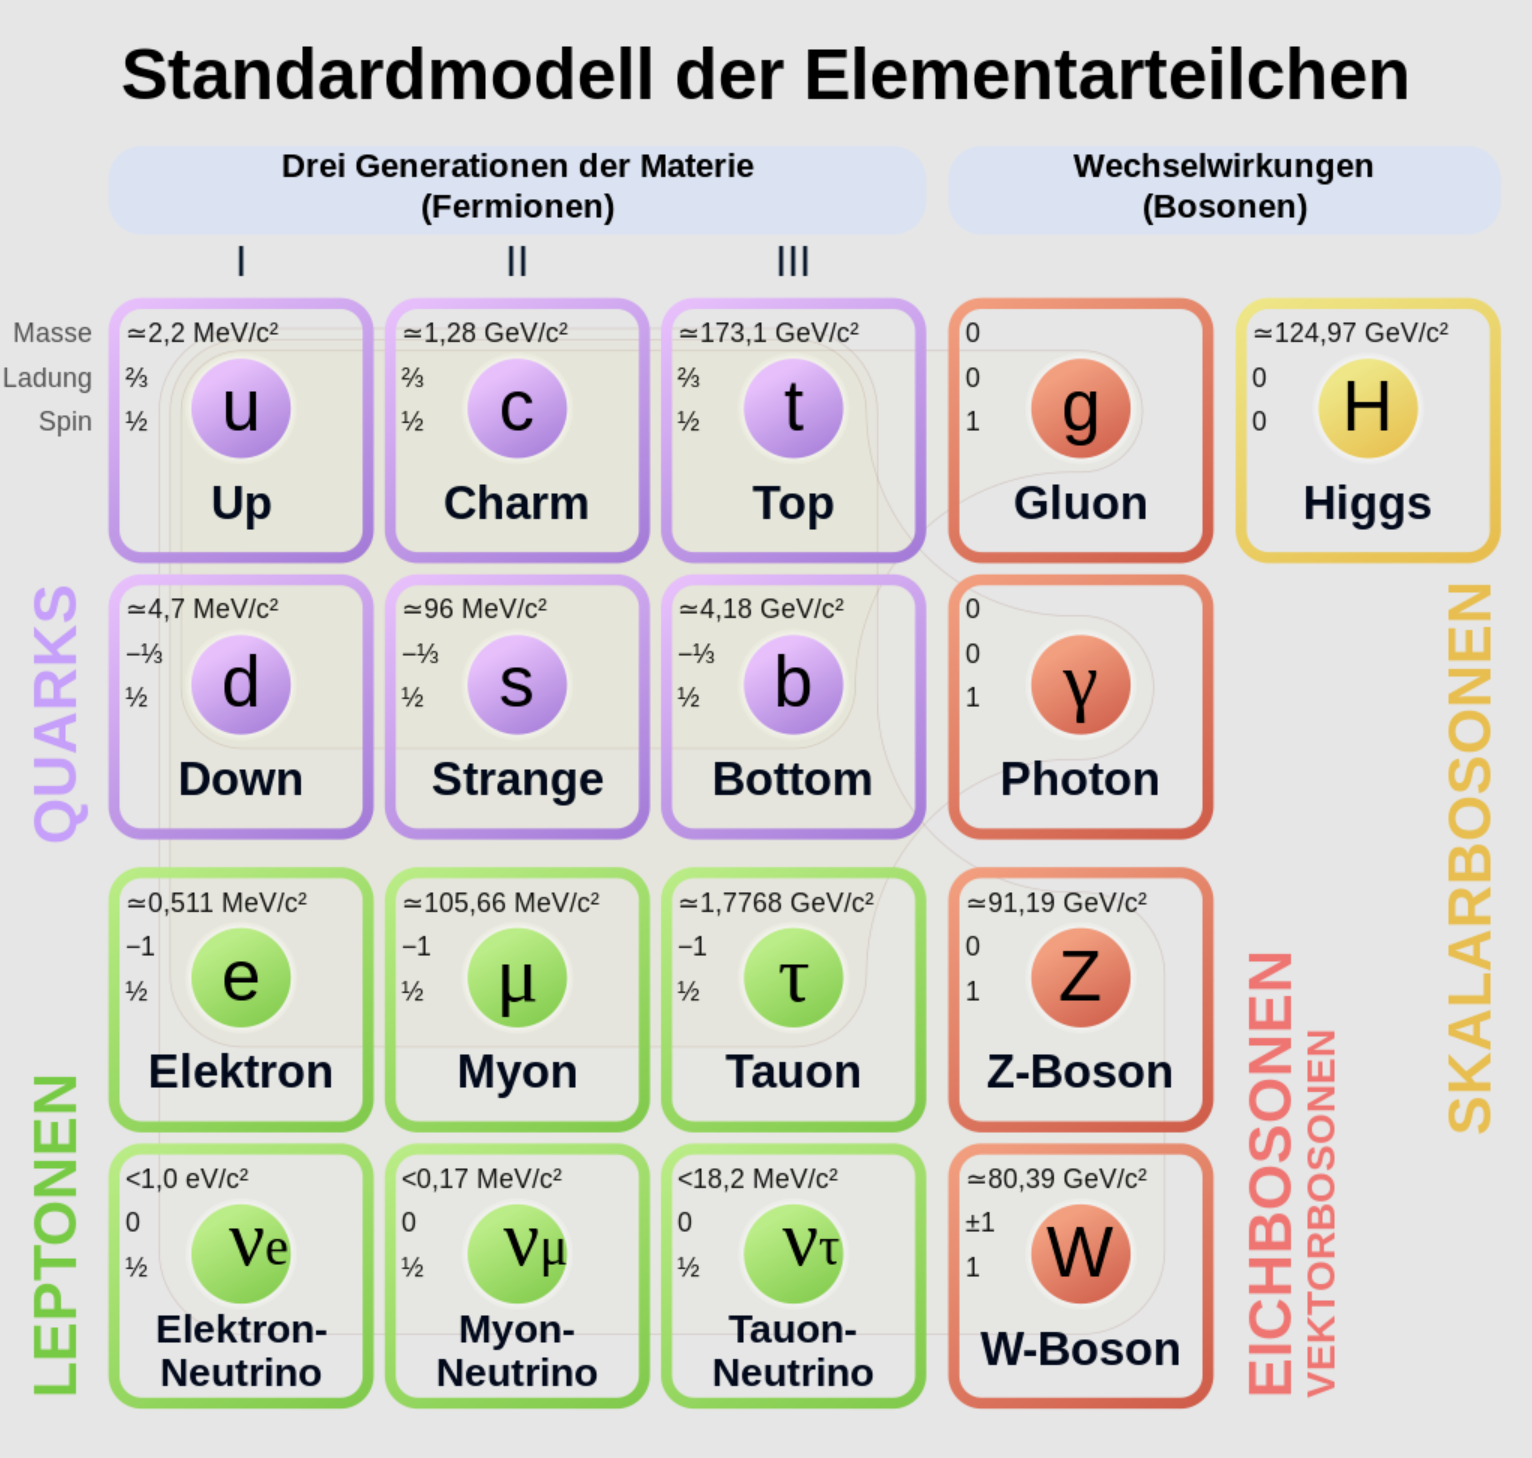
\includegraphics[width=0.4\textwidth]{images:/standartmodell.png}
    \caption{ Standardmodell der Teilchenphysik   \cite{standardmodell}.}
    \label{standartmodell}
\end{figure}




\subsection{Entstehung kosmischer Myonen} \label{myon_entstehung}
Myonen sind ein Produkt der Zerfallskette der sekundären kosmischen Strahlung. Wie der Name vermuten lässt ist diese Folge der Interaktion primärer kosmischer Strahlung mit der oberen Erdatmosphäre.
Hier Wechselwirken diese hochenergetischen Protonen mit den Atomen der Atmosphäre.
Da bei entstehen Pionen, Kaonen und Nukleonen. 
Es gibt 3 verschiedene Pionen, 2 geladene $\pi^{\pm}$ und ein neutrales $\pi^0$. 
Die geladenen Pionen zerfallen in Myonen und ihr entsprechendes Neutrino gemäß 
\begin{align}
    \pi^+ \rightarrow  \mu^+ + \nu_{\mu},\\
    \pi^- \rightarrow  \mu^- + \overline{\nu}_{\mu}.
\end{align} 
Das $\pi^0$ zerfällt in den meisten Fällen in zwei Gammaquanten, oder in ein Positron, ein Elektron und ein Gamma Quant.\\
Bei den Kaonen entstehen Myonen nur in einem der Zerfallsrozesse.
Dies ist beim $K^-$ der Fall.
Es gilt 
\begin{equation}
    K^- \rightarrow \mu^- + \overline{\nu}_{\mu}.
\end{equation}
\\
\newline

Da Myonen sich mit annähernd Lichtgeschwindigkeit bewegen unterliegen sie der speziellen Relativitätstheorie. 
Aus diesem Grund können überhaut erst aussreichend Myonen auf Meereshöhe gemessen werden. 
Wäre es nicht um die Zeitdilatation, welche die Myonen erfahren, würden diese bereits nach kurzer Distanz wieder zerfallen sein. %Muss das hier genauer ausgeführt werden
Der Fluss von Myonen auf Meereshöhe liegt ca. bei einem Teilchen pro $cm^2/min$. % Muss ich hierfür eine Quelle angeben?


\begin{figure}[H]
    \centering
    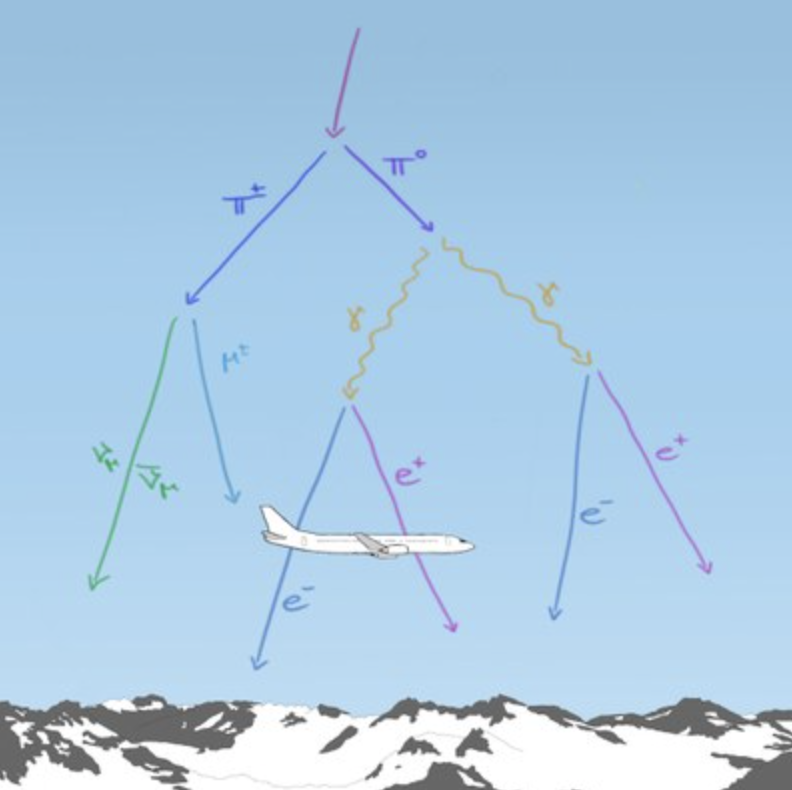
\includegraphics[width=0.4\textwidth]{images:/strahlung.png}
    \caption{ Teilchenkaskade der sekundären Höhenstrahlung   \cite{höhenstrahlung}.}
    \label{höhen:pic}
\end{figure}



\subsection{Dämpfung von Myonen Durch Blei}



\subsection{Myonen Silizium Interaktion}



\subsection{HV MAPS Sensor und Auslese}
\clearpage


\section{Experimenteller Aufbau und Durchführung}
\clearpage


\section{Ergebnisse}
\clearpage


\section{Fazit}
\clearpage




\printbibliography[title = Literaturverzeichnis, heading = bibintoc]
\clearpage

\appendix
\input{anhang}


\end{document}